	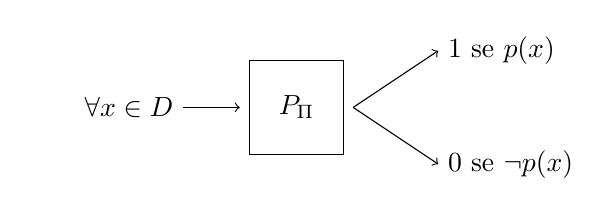
\begin{tikzpicture}[scale=1.2]
	\draw[->] (2.3,1.5) node[left]{$\forall x \in D$} -- (2.9,1.5);
	\node[left] at (2.3,1.5) {$\phantom{cod(P)=n}$};
	\draw (3,2) rectangle (4,1);
	\node at (3.5,1.5) {$P_\Pi$};
	\draw[->] (4.1,1.5) -- (5,2.1) node [right] {$1$ se $p(x)$};
	\draw[->] (4.1,1.5) -- (5,0.9) node [right] {$0$ se $\neg p(x)$};
\end{tikzpicture}